% --------------------------------------------	
% This is an example 					
% Adding a customization Layer			
% Autogenerated LaTeX file for books 			
% --------------------------------------------	
\documentclass[spanish,french,english,a4paper,10pt,final]{report}
\label{book}\usepackage{ifthen}
% --------------------------------------------
% Check for PDFLaTeX/LaTeX 
% --------------------------------------------
\newif\ifpdf
\ifx\pdfoutput\undefined
\pdffalse % we are not running PDFLaTeX
\else
\pdfoutput=1 % we are running PDFLaTeX
\pdftrue
\fi
% --------------------------------------------
% Load graphicx package with pdf if needed 
% --------------------------------------------
\ifpdf
\usepackage[pdftex]{graphicx}
\pdfcompresslevel=9
\else
\usepackage{graphicx}
\fi
\usepackage{anysize}
\marginsize{3cm}{2cm}{1.25cm}{1.25cm}
% ---------------------- 
% Most Common Packages   
% ---------------------- 
\usepackage{makeidx} 
\usepackage{varioref}         
\usepackage{latexsym}         
\usepackage{enumerate}         
\usepackage{fancybox}      
\usepackage{float}       
\usepackage{ragged2e}       
\usepackage[french]{babel} 
\usepackage{isolatin1}         
\usepackage{rotating}         
\usepackage{subfigure}         
\usepackage{tabularx}         
\usepackage{url}         
% ---------------
% Document Font  
% ---------------
\usepackage{palatino}
 \def\keywords{\vspace{-.3em}
 \if@twocolumn
 \small{\itshape 
Keywords }\/\bfseries---$\!$%
 \else
 \begin{center}\small\bfseries 
Keywords \end{center}\quotation\small
 \fi}
 \def\endkeywords{\vspace{0.6em}\par\if@twocolumn\else\endquotation\fi
 \normalsize\rmfamily}
% ---------------------------------------------- 
% Define a new LaTeX environment (adminipage)    
% ---------------------------------------------- 
\newenvironment{admminipage}%
{ % this code corresponds to the \begin{adminipage} command
 \begin{Sbox}%
 \begin{minipage}%
} %done
{ % this code corresponds to the \end{adminipage} command
 \end{minipage}
 \end{Sbox}
 \fbox{\TheSbox}
} %done
% ---------------------------------------------- 
% Define a new LaTeX length (admlength)          
% ---------------------------------------------- 
\newlength{\admlength}
% ---------------------------------------------- 
% Define a new LaTeX environment (admonition)    
% With 2 parameters:                             
% #1 The file (e.g. note.pdf)                    
% #2 The caption                                 
% ---------------------------------------------- 
\newenvironment{admonition}[2] 
{ % this code corresponds to the \begin{admonition} command
 \hspace{0mm}\newline\hspace*\fill\newline
 \noindent
 \setlength{\fboxsep}{5pt}
 \setlength{\admlength}{\linewidth}
 \addtolength{\admlength}{-10\fboxsep}
 \addtolength{\admlength}{-10\fboxrule}
 \admminipage{\admlength}
 {\bfseries \sc\large{#2}} \newline
 \\[1mm]
 \sffamily
 \includegraphics[width=1cm]{#1}
 \addtolength{\admlength}{-1cm}
 \addtolength{\admlength}{-20pt}
 \begin{minipage}[lt]{\admlength}
 \parskip=0.5\baselineskip \advance\parskip by 0pt plus 2pt
} %done
{ % this code corresponds to the \end{admonition} command
 \vspace{5mm} 
 \end{minipage}
 \endadmminipage
 \vspace{.5em}
 \par
}
% --------------------------------------------
% Commands to manage/style/create floats      
% figures, tables, algorithms, examples, eqn  
% --------------------------------------------
 \floatstyle{ruled}
 \restylefloat{figure}
 \floatstyle{ruled}
 \restylefloat{table}
 \floatstyle{ruled}
 \newfloat{program}{ht}{lop}[section]
 \floatstyle{ruled}
 \newfloat{example}{ht}{loe}[section]
 \floatname{example}{Example}
 \floatstyle{ruled}
 \newfloat{dbequation}{ht}{loe}[section]
 \floatname{dbequation}{Equation}
 \floatstyle{boxed}
 \newfloat{algorithm}{ht}{loa}[section]
 \floatname{algorithm}{Algorithm}
\ifpdf
\DeclareGraphicsExtensions{.pdf,.png,.jpg}
\else
\DeclareGraphicsExtensions{.eps}
\fi
% --------------------------------------------
% $latex.caption.swapskip enabled for $formal.title.placement support
\newlength{\docbooktolatextempskip}
\newcommand{\captionswapskip}{\setlength{\docbooktolatextempskip}{\abovecaptionskip}\setlength{\abovecaptionskip}{\belowcaptionskip}\setlength{\belowcaptionskip}{\docbooktolatextempskip}}
% --------------------------------------------
\makeatletter
\newcommand{\href}[1]{{}}
\newcommand{\hyperlink}[1]{{}}
\newcommand{\hypertarget}[2]{#2}

\def\docbooktolatexgobble{\expandafter\@gobble}
% Facilitate use of \cite with \label
\newcommand{\docbooktolatexbibaux}[2]{%
  \protected@write\@auxout{}{\string\global\string\@namedef{docbooktolatexcite@#1}{#2}}
}
\newcommand{\docbooktolatexcite}[2]{%
  \@ifundefined{docbooktolatexcite@#1}%
  {\cite{#1}}%
  {\def\@docbooktolatextemp{#2}\ifx\@docbooktolatextemp\@empty%
   \cite{\@nameuse{docbooktolatexcite@#1}}%
   \else\cite[#2]{\@nameuse{docbooktolatexcite@#1}}%
   \fi%
  }%
}
\newcommand{\docbooktolatexbackcite}[1]{%
  \ifx\Hy@backout\@undefined\else%
    \@ifundefined{docbooktolatexcite@#1}{%
      % emit warning?
    }{%
      \ifBR@verbose%
        \PackageInfo{backref}{back cite \string`#1\string' as \string`\@nameuse{docbooktolatexcite@#1}\string'}%
      \fi%
      \Hy@backout{\@nameuse{docbooktolatexcite@#1}}%
    }%
  \fi%
}
% --------------------------------------------
% A way to honour <footnoteref>s
% Blame j-devenish (at) users.sourceforge.net
% In any other LaTeX context, this would probably go into a style file.
\newcommand{\docbooktolatexusefootnoteref}[1]{\@ifundefined{@fn@label@#1}%
  {\hbox{\@textsuperscript{\normalfont ?}}%
    \@latex@warning{Footnote label `#1' was not defined}}%
  {\@nameuse{@fn@label@#1}}}
\newcommand{\docbooktolatexmakefootnoteref}[1]{%
  \protected@write\@auxout{}%
    {\global\string\@namedef{@fn@label@#1}{\@makefnmark}}%
  \@namedef{@fn@label@#1}{\hbox{\@textsuperscript{\normalfont ?}}}%
  }
% --------------------------------------------
% Hacks for honouring row/entry/@align
% (\hspace not effective when in paragraph mode)
% Naming convention for these macros is:
% 'docbooktolatex' 'align' {alignment-type} {position-within-entry}
% where r = right, l = left, c = centre
\newcommand{\docbooktolatexalignrl}{\protect\ifvmode\raggedleft\else\hfill\fi}
\newcommand{\docbooktolatexalignrr}{\protect}
\newcommand{\docbooktolatexalignll}{\protect\ifvmode\raggedright\else\fi}
\newcommand{\docbooktolatexalignlr}{\protect\ifvmode\else\hspace*\fill\fi}
\newcommand{\docbooktolatexaligncl}{\protect\ifvmode\centering\else\hfill\fi}
\newcommand{\docbooktolatexaligncr}{\protect\ifvmode\else\hspace*\fill\fi}
\ifx\captionswapskip\@undefined\newcommand{\captionswapskip}{}\fi
\makeatother
\title{\bfseries The Subfigure option}
\author{Ramon Casellas}
% --------------------------------------------
\makeindex
\makeglossary
% --------------------------------------------

\setcounter{tocdepth}{4}

\setcounter{secnumdepth}{4}
\begin{document}

\InputIfFileExists{title}{\typeout{WARNING: Using cover pagetitle}}{\maketitle\pagestyle{plain}\thispagestyle{empty}}



\noindent{\bfseries A simple figure } \\ 
\label{id174292}
 jsdlkfj lsjd jsdkfjlksdfj lkjdsf lj sdlfj lksdj fljdslk jlksdjf lkjdsf ljsdlk fj
dsfkjsd lkfjklsdjf lkjs dfj lkjsd flkj sdlkj lkmjs dflkj sdlfj lmksjd flkj lksdjf 
dsfkjsd lkfjklsdjf lkjs dfj lkjsd flkj sdlkj lkmjs dflkj sdlfj lmksjd flkj lksdjf 
dsfkjsd lkfjklsdjf lkjs dfj lkjsd flkj sdlkj lkmjs dflkj sdlfj lmksjd flkj lksdjf 
dsfkjsd lkfjklsdjf lkjs dfj lkjsd flkj sdlkj lkmjs dflkj sdlfj lmksjd flkj lksdjf 
dsfkjsd lkfjklsdjf lkjs dfj lkjsd flkj sdlkj lkmjs dflkj sdlfj lmksjd flkj lksdjf 
sdflj lkjsdf mklj sdkfklj jdsfklj dsflj sdfjklsjd lkj sdklj lkjlk jsdlfj lksj flj 
dsfkjsd lkfjklsdjf lkjs dfj lkjsd flkj sdlkj lkmjs dflkj sdlfj lmksjd flkj lksdjf 
dsfkjsd lkfjklsdjf lkjs dfj lkjsd flkj sdlkj lkmjs dflkj sdlfj lmksjd flkj lksdjf 
sdflj lkjsdf mklj sdkfklj jdsfklj dsflj sdfjklsjd lkj sdklj lkjlk jsdlfj lksj flj 


% figure ------------------------------------------------------
\begin{figure}[hbt]
\begin{center}%
\hypertarget{fig1}{}%

{{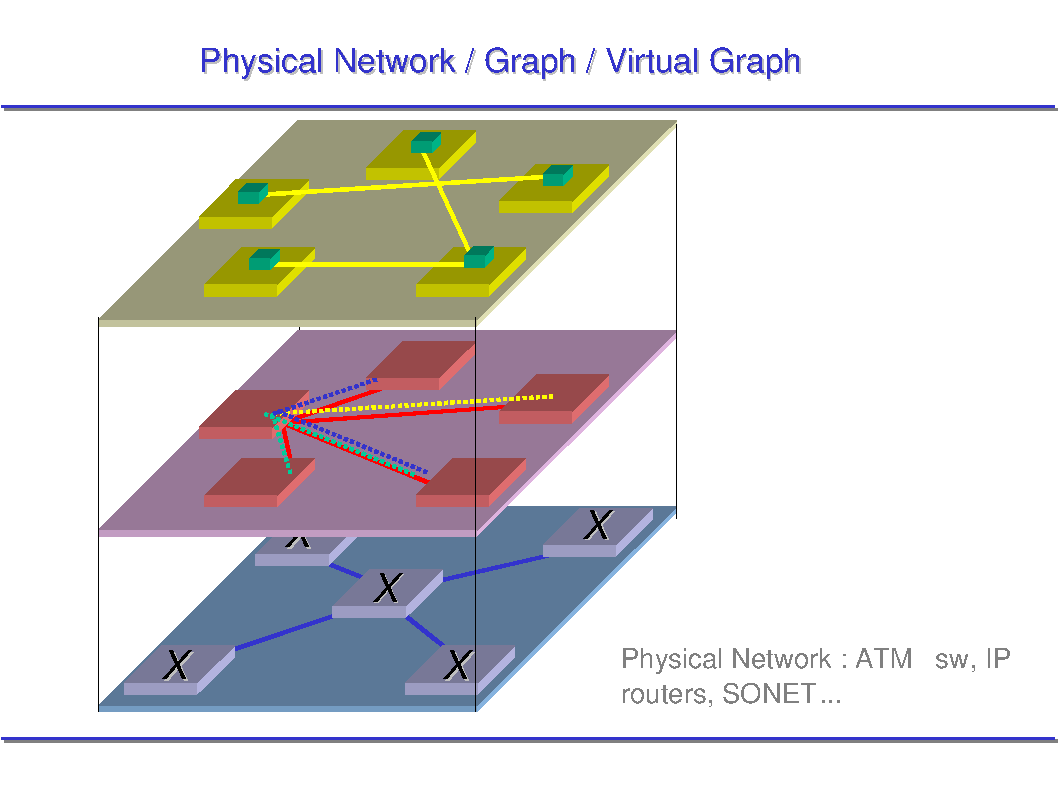
\includegraphics[scale=0.67]{figures/sample}}}
\caption{{{A pdf/eps fig scaled to 67\% and centred}}. 
This is the caption (next to the title).
}
\label{fig1}
\end{center}
\end{figure}


 jsdlkfj lsjd jsdkfjlksdfj lkjdsf lj sdlfj lksdj fljdslk jlksdjf lkjdsf ljsdlk fj
dsfkjsd lkfjklsdjf lkjs dfj lkjsd flkj sdlkj lkmjs dflkj sdlfj lmksjd flkj lksdjf 
dsfkjsd lkfjklsdjf lkjs dfj lkjsd flkj sdlkj lkmjs dflkj sdlfj lmksjd flkj lksdjf 
dsfkjsd lkfjklsdjf lkjs dfj lkjsd flkj sdlkj lkmjs dflkj sdlfj lmksjd flkj lksdjf 
dsfkjsd lkfjklsdjf lkjs dfj lkjsd flkj sdlkj lkmjs dflkj sdlfj lmksjd flkj lksdjf 
dsfkjsd lkfjklsdjf lkjs dfj lkjsd flkj sdlkj lkmjs dflkj sdlfj lmksjd flkj lksdjf 
sdflj lkjsdf mklj sdkfklj jdsfklj dsflj sdfjklsjd lkj sdklj lkjlk jsdlfj lksj flj 
dsfkjsd lkfjklsdjf lkjs dfj lkjsd flkj sdlkj lkmjs dflkj sdlfj lmksjd flkj lksdjf 
dsfkjsd lkfjklsdjf lkjs dfj lkjsd flkj sdlkj lkmjs dflkj sdlfj lmksjd flkj lksdjf 
sdflj lkjsdf mklj sdkfklj jdsfklj dsflj sdfjklsjd lkj sdklj lkjlk jsdlfj lksj flj 


 jsdlkfj lsjd jsdkfjlksdfj lkjdsf lj sdlfj lksdj fljdslk jlksdjf lkjdsf ljsdlk fj
dsfkjsd lkfjklsdjf lkjs dfj lkjsd flkj sdlkj lkmjs dflkj sdlfj lmksjd flkj lksdjf 
dsfkjsd lkfjklsdjf lkjs dfj lkjsd flkj sdlkj lkmjs dflkj sdlfj lmksjd flkj lksdjf 
dsfkjsd lkfjklsdjf lkjs dfj lkjsd flkj sdlkj lkmjs dflkj sdlfj lmksjd flkj lksdjf 
dsfkjsd lkfjklsdjf lkjs dfj lkjsd flkj sdlkj lkmjs dflkj sdlfj lmksjd flkj lksdjf 
dsfkjsd lkfjklsdjf lkjs dfj lkjsd flkj sdlkj lkmjs dflkj sdlfj lmksjd flkj lksdjf 
sdflj lkjsdf mklj sdkfklj jdsfklj dsflj sdfjklsjd lkj sdklj lkjlk jsdlfj lksj flj 
dsfkjsd lkfjklsdjf lkjs dfj lkjsd flkj sdlkj lkmjs dflkj sdlfj lmksjd flkj lksdjf 
dsfkjsd lkfjklsdjf lkjs dfj lkjsd flkj sdlkj lkmjs dflkj sdlfj lmksjd flkj lksdjf 
sdflj lkjsdf mklj sdkfklj jdsfklj dsflj sdfjklsjd lkj sdklj lkjlk jsdlfj lksj flj 




\noindent{\bfseries The subfig package !!!!!!} \\ 
\label{id173057}
 jsdlkfj lsjd jsdkfjlksdfj lkjdsf lj sdlfj lksdj fljdslk jlksdjf lkjdsf ljsdlk fj
dsfkjsd lkfjklsdjf lkjs dfj lkjsd flkj sdlkj lkmjs dflkj sdlfj lmksjd flkj lksdjf 
dsfkjsd lkfjklsdjf lkjs dfj lkjsd flkj sdlkj lkmjs dflkj sdlfj lmksjd flkj lksdjf 
dsfkjsd lkfjklsdjf lkjs dfj lkjsd flkj sdlkj lkmjs dflkj sdlfj lmksjd flkj lksdjf 
dsfkjsd lkfjklsdjf lkjs dfj lkjsd flkj sdlkj lkmjs dflkj sdlfj lmksjd flkj lksdjf 
sdflj lkjsdf mklj sdkfklj jdsfklj dsflj sdfjklsjd lkj sdklj lkjlk jsdlfj lksj flj 
dsfkjsd lkfjklsdjf lkjs dfj lkjsd flkj sdlkj lkmjs dflkj sdlfj lmksjd flkj lksdjf 
sdflj lkjsdf mklj sdkfklj jdsfklj dsflj sdfjklsjd lkj sdklj lkjlk jsdlfj lksj flj 
sdflj lkjsdf mklj sdkfklj jdsfklj dsflj sdfjklsjd lkj sdklj lkjlk jsdlfj lksj flj 
sdflj lkjsdf mklj sdkfklj jdsfklj dsflj sdfjklsjd lkj sdklj lkjlk jsdlfj lksj flj 
sdflj lkjsdf mklj sdkfklj jdsfklj dsflj sdfjklsjd lkj sdklj lkjlk jsdlfj lksj flj 
sdflj lkjsdf mklj sdkfklj jdsfklj dsflj sdfjklsjd lkj sdklj lkjlk jsdlfj lksj flj 


% figure ------------------------------------------------------
\begin{figure}[hbt]
\begin{center}%
\hypertarget{fig2}{}%

{\subfigure[]{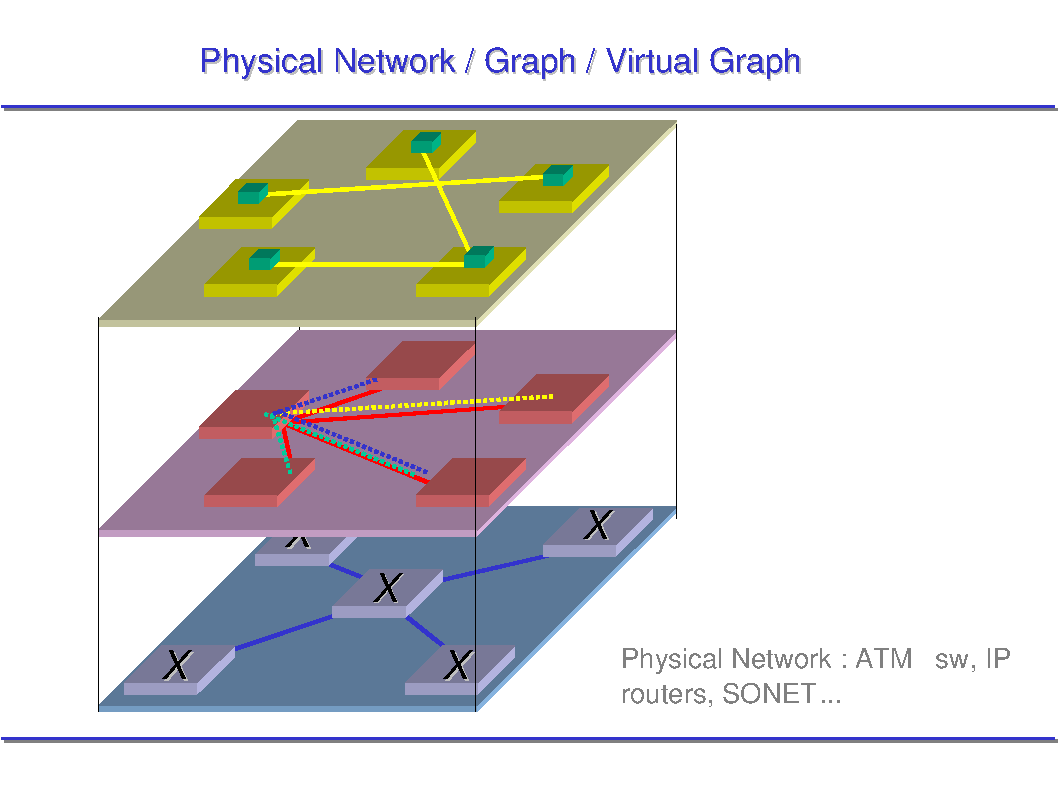
\includegraphics[scale=0.4]{figures/sample}}}
\caption{{{ LOOK WHAT HAPPENS WHEN YOU PUT SEVERAL IMAGEOBJECT IN ONE MEDIAOBJECT !!! }}. 
This is a worst-case scenario and the first imageobject should be picked by default. It should not have a subcaption label.
}
\label{fig2}
\end{center}
\end{figure}


 jsdlkfj lsjd jsdkfjlksdfj lkjdsf lj sdlfj lksdj fljdslk jlksdjf lkjdsf ljsdlk fj
dsfkjsd lkfjklsdjf lkjs dfj lkjsd flkj sdlkj lkmjs dflkj sdlfj lmksjd flkj lksdjf 
dsfkjsd lkfjklsdjf lkjs dfj lkjsd flkj sdlkj lkmjs dflkj sdlfj lmksjd flkj lksdjf 
dsfkjsd lkfjklsdjf lkjs dfj lkjsd flkj sdlkj lkmjs dflkj sdlfj lmksjd flkj lksdjf 
dsfkjsd lkfjklsdjf lkjs dfj lkjsd flkj sdlkj lkmjs dflkj sdlfj lmksjd flkj lksdjf 
sdflj lkjsdf mklj sdkfklj jdsfklj dsflj sdfjklsjd lkj sdklj lkjlk jsdlfj lksj flj 
dsfkjsd lkfjklsdjf lkjs dfj lkjsd flkj sdlkj lkmjs dflkj sdlfj lmksjd flkj lksdjf 
sdflj lkjsdf mklj sdkfklj jdsfklj dsflj sdfjklsjd lkj sdklj lkjlk jsdlfj lksj flj 
sdflj lkjsdf mklj sdkfklj jdsfklj dsflj sdfjklsjd lkj sdklj lkjlk jsdlfj lksj flj 
sdflj lkjsdf mklj sdkfklj jdsfklj dsflj sdfjklsjd lkj sdklj lkjlk jsdlfj lksj flj 
sdflj lkjsdf mklj sdkfklj jdsfklj dsflj sdfjklsjd lkj sdklj lkjlk jsdlfj lksj flj 


% figure ------------------------------------------------------
\begin{figure}[hbt]
\begin{center}%
\hypertarget{fig3}{}%

{\subfigure[Caption one.]{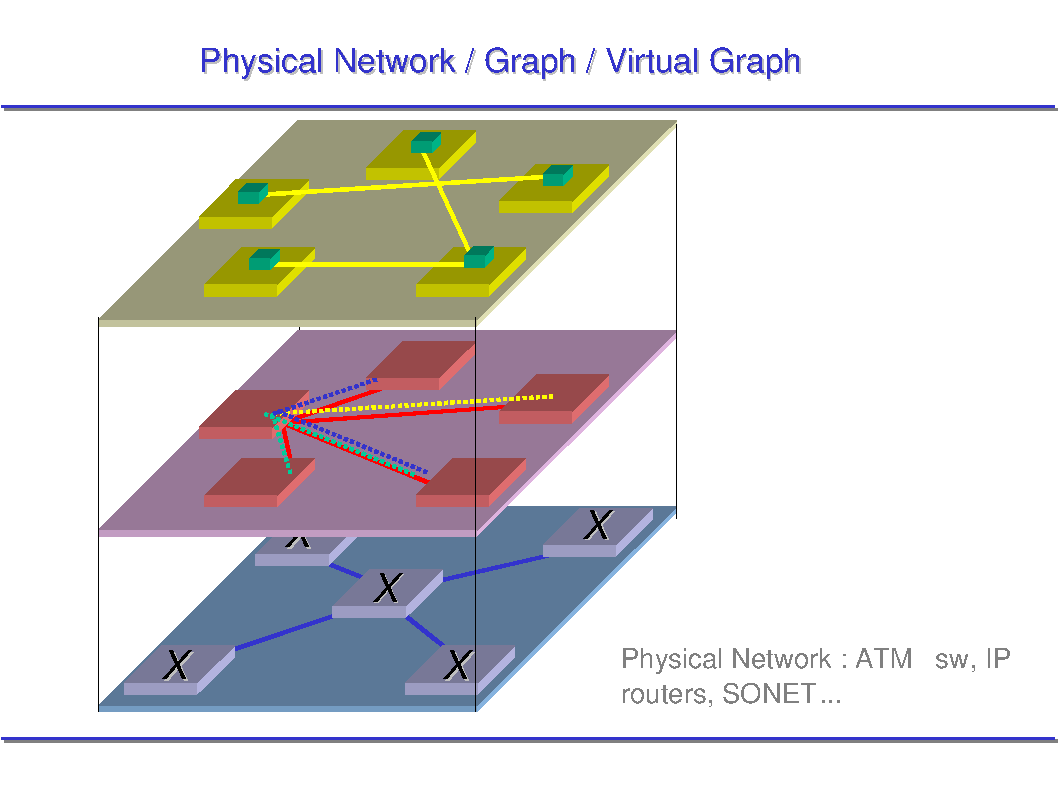
\includegraphics[scale=0.4]{figures/sample}}}
{\subfigure[Caption two.]{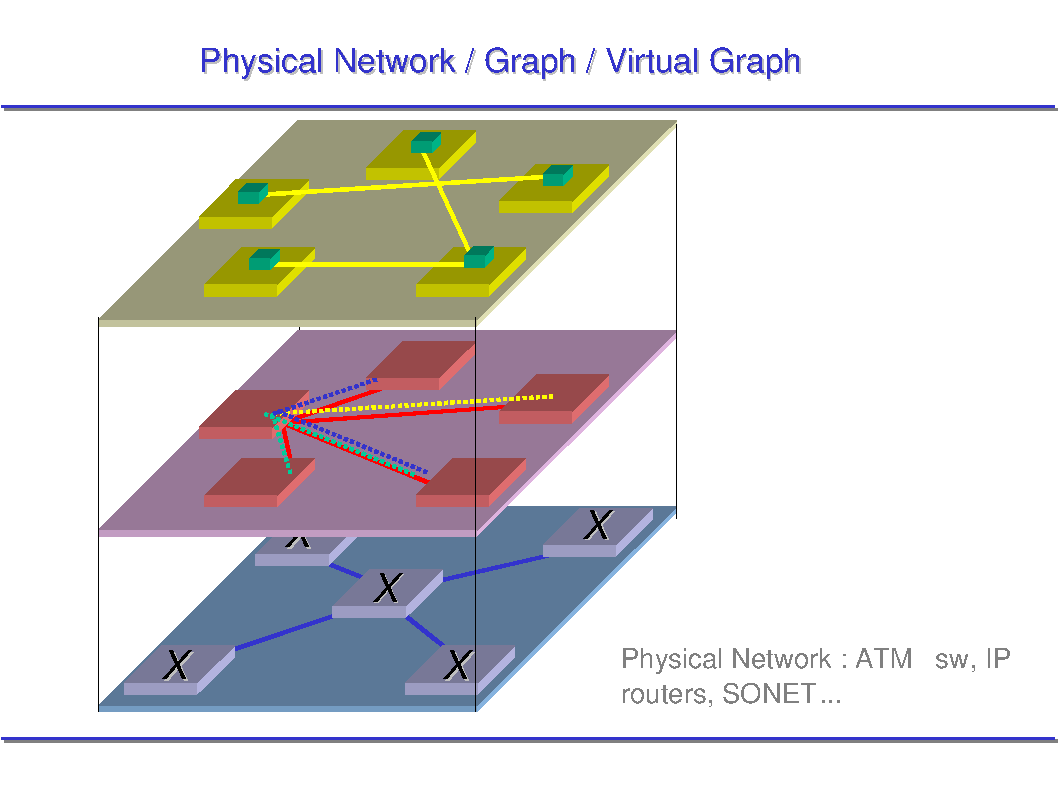
\includegraphics[scale=0.4]{figures/sample}}}
\caption{{{ Look what happens when you put several mediaobject in one figure. }}}
\label{fig3}
\end{center}
\end{figure}


 jsdlkfj lsjd jsdkfjlksdfj lkjdsf lj sdlfj lksdj fljdslk jlksdjf lkjdsf ljsdlk fj
dsfkjsd lkfjklsdjf lkjs dfj lkjsd flkj sdlkj lkmjs dflkj sdlfj lmksjd flkj lksdjf 
dsfkjsd lkfjklsdjf lkjs dfj lkjsd flkj sdlkj lkmjs dflkj sdlfj lmksjd flkj lksdjf 
dsfkjsd lkfjklsdjf lkjs dfj lkjsd flkj sdlkj lkmjs dflkj sdlfj lmksjd flkj lksdjf 
dsfkjsd lkfjklsdjf lkjs dfj lkjsd flkj sdlkj lkmjs dflkj sdlfj lmksjd flkj lksdjf 
sdflj lkjsdf mklj sdkfklj jdsfklj dsflj sdfjklsjd lkj sdklj lkjlk jsdlfj lksj flj 
dsfkjsd lkfjklsdjf lkjs dfj lkjsd flkj sdlkj lkmjs dflkj sdlfj lmksjd flkj lksdjf 
sdflj lkjsdf mklj sdkfklj jdsfklj dsflj sdfjklsjd lkj sdklj lkjlk jsdlfj lksj flj 
sdflj lkjsdf mklj sdkfklj jdsfklj dsflj sdfjklsjd lkj sdklj lkjlk jsdlfj lksj flj 
sdflj lkjsdf mklj sdkfklj jdsfklj dsflj sdfjklsjd lkj sdklj lkjlk jsdlfj lksj flj 
sdflj lkjsdf mklj sdkfklj jdsfklj dsflj sdfjklsjd lkj sdklj lkjlk jsdlfj lksj flj 


% figure ------------------------------------------------------
\begin{figure}[hbt]
\begin{center}%
\hypertarget{fig4}{}%

{\subfigure[This should show imagedata.]{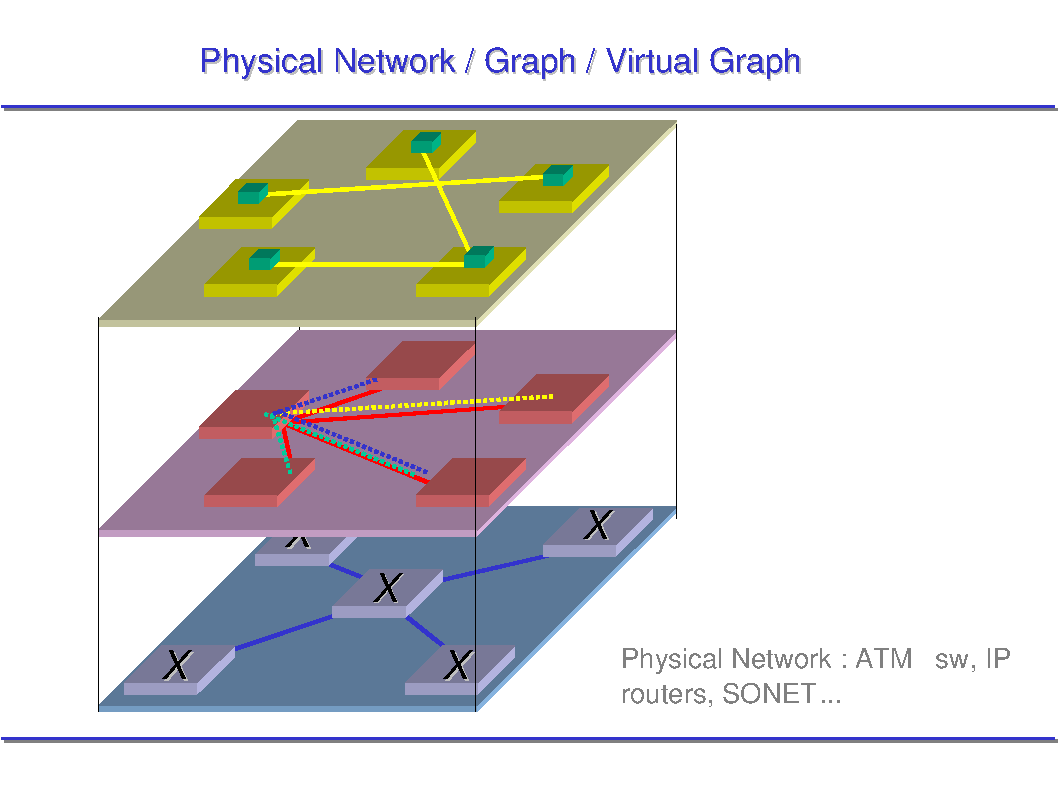
\includegraphics[scale=0.4]{figures/sample}}}
{\subfigure[The correct imagedata format should have been chosen.]{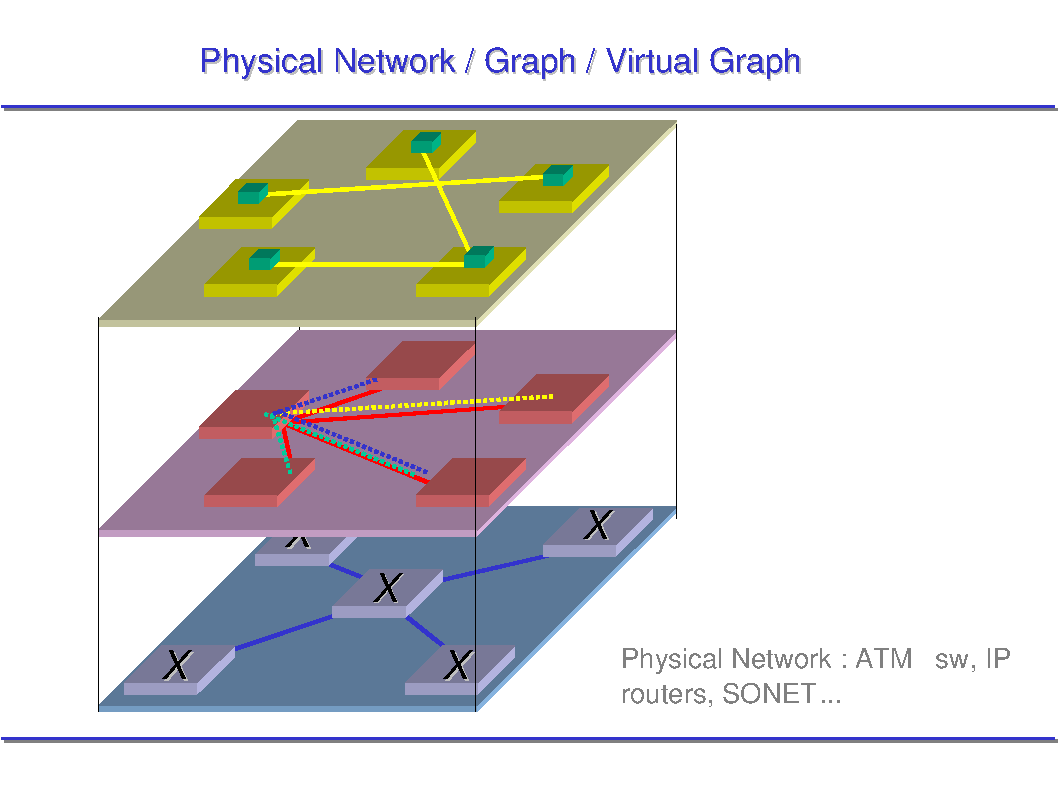
\includegraphics[scale=0.4]{figures/sample.pdf}}}
{\subfigure[This should be graphical.]{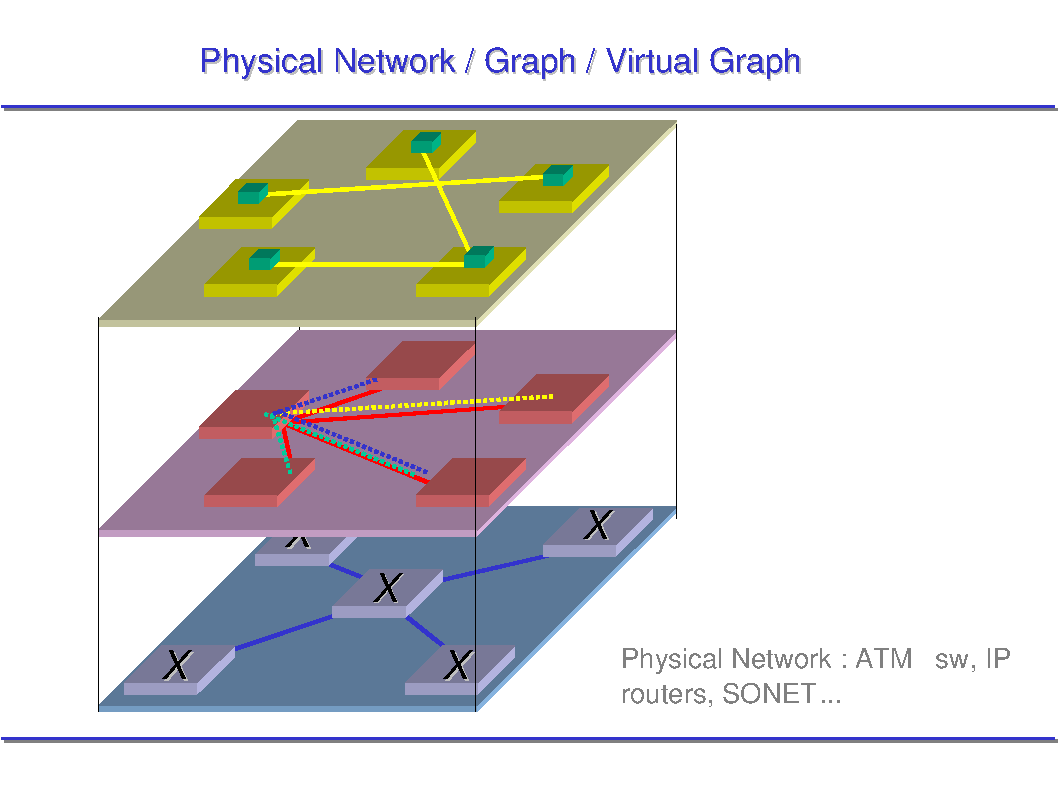
\includegraphics[scale=0.4]{figures/sample}}}
A textobject.
\caption{{{ This should have chosen the correct imageobject in each case }}}
\label{fig4}
\end{center}
\end{figure}


 jsdlkfj lsjd jsdkfjlksdfj lkjdsf lj sdlfj lksdj fljdslk jlksdjf lkjdsf ljsdlk fj
dsfkjsd lkfjklsdjf lkjs dfj lkjsd flkj sdlkj lkmjs dflkj sdlfj lmksjd flkj lksdjf 
dsfkjsd lkfjklsdjf lkjs dfj lkjsd flkj sdlkj lkmjs dflkj sdlfj lmksjd flkj lksdjf 
dsfkjsd lkfjklsdjf lkjs dfj lkjsd flkj sdlkj lkmjs dflkj sdlfj lmksjd flkj lksdjf 
dsfkjsd lkfjklsdjf lkjs dfj lkjsd flkj sdlkj lkmjs dflkj sdlfj lmksjd flkj lksdjf 
sdflj lkjsdf mklj sdkfklj jdsfklj dsflj sdfjklsjd lkj sdklj lkjlk jsdlfj lksj flj 
dsfkjsd lkfjklsdjf lkjs dfj lkjsd flkj sdlkj lkmjs dflkj sdlfj lmksjd flkj lksdjf 
sdflj lkjsdf mklj sdkfklj jdsfklj dsflj sdfjklsjd lkj sdklj lkjlk jsdlfj lksj flj 
sdflj lkjsdf mklj sdkfklj jdsfklj dsflj sdfjklsjd lkj sdklj lkjlk jsdlfj lksj flj 
sdflj lkjsdf mklj sdkfklj jdsfklj dsflj sdfjklsjd lkj sdklj lkjlk jsdlfj lksj flj 
sdflj lkjsdf mklj sdkfklj jdsfklj dsflj sdfjklsjd lkj sdklj lkjlk jsdlfj lksj flj 


% figure ------------------------------------------------------
\begin{figure}[hbt]
\begin{center}%
\hypertarget{fig5}{}%

{\subfigure[]{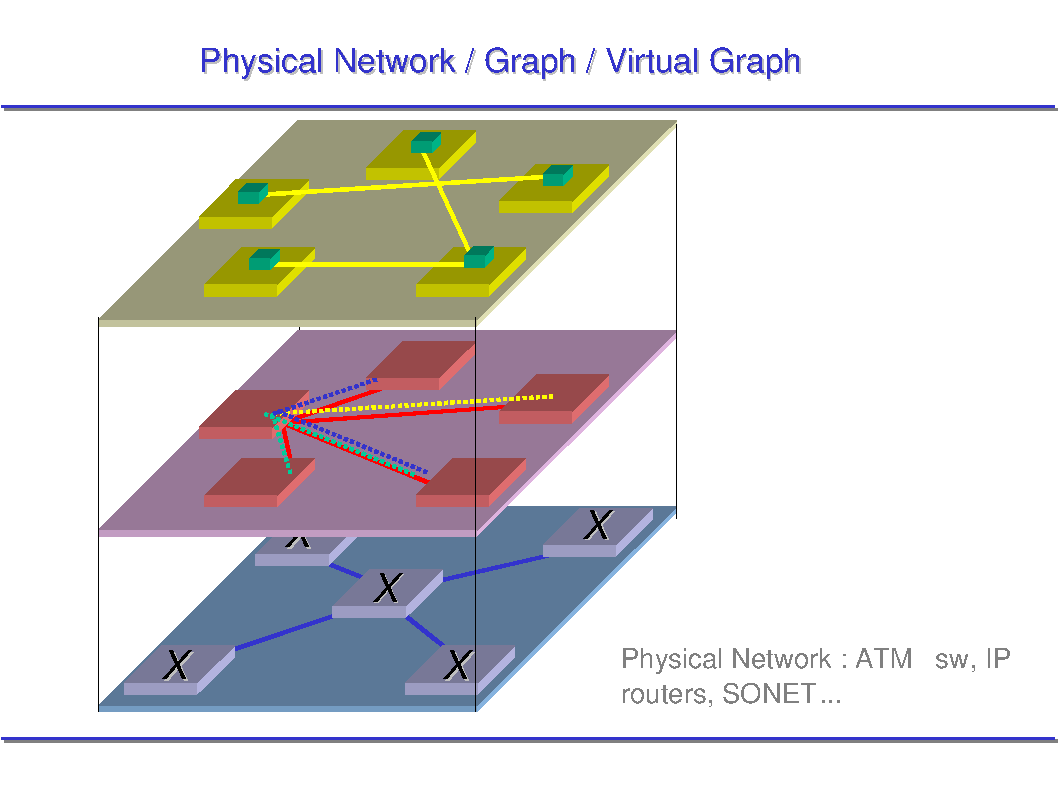
\includegraphics[scale=0.4]{figures/sample}}}
\caption{{{ Another test }}. 
This should be graphical. It should not have a subcaption label.
}
\label{fig5}
\end{center}
\end{figure}


% figure ------------------------------------------------------
\begin{figure}[hbt]
\begin{center}%
\hypertarget{fig6}{}%

{\subfigure[]{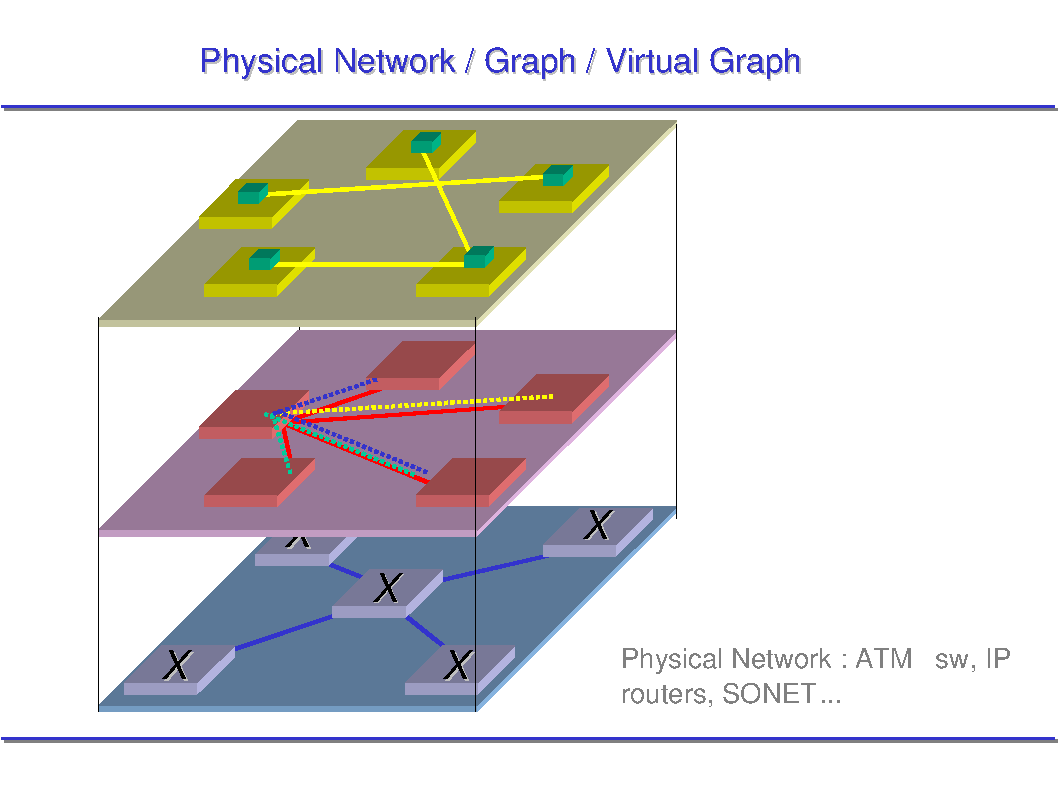
\includegraphics[scale=0.09]{figures/sample}}}
\caption{{{ Another test }}. 
This should be graphical, 9\% of original size. It should not have a subcaption label.
}
\label{fig6}
\end{center}
\end{figure}


This:
        {{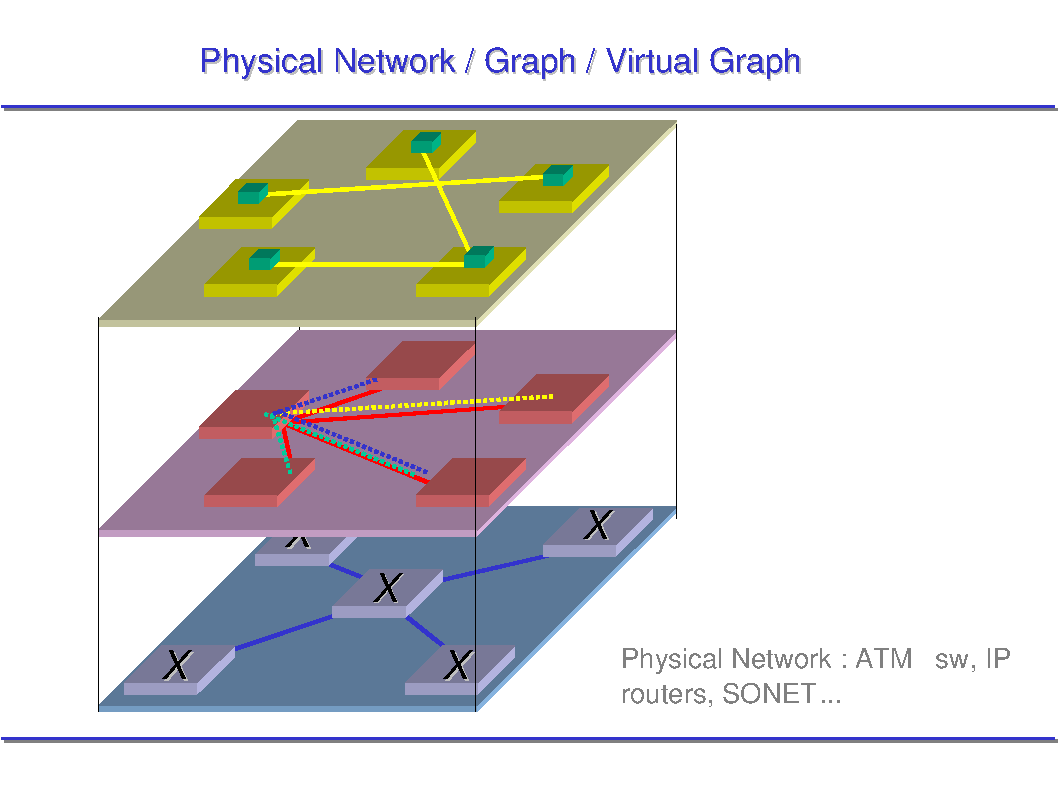
\includegraphics[scale=0.09]{figures/sample}}}
is an {\texttt{{inlinemediaobject}}}.

\end{document}

